\documentclass[12pt,a4paper]{article}
\usepackage[utf8]{inputenc}
\usepackage{amsmath}
\usepackage{amssymb}
\usepackage{tikz}
\usetikzlibrary{shapes,arrows,positioning,calc}
\usepackage{geometry}
\usepackage{listings}
\usepackage{xcolor}
\usepackage{fancyhdr}
\usepackage{graphicx}

\geometry{margin=1in}

% Code listing style
\lstdefinestyle{javaStyle}{
    language=Java,
    basicstyle=\ttfamily\footnotesize,
    keywordstyle=\color{blue}\bfseries,
    commentstyle=\color{gray}\itshape,
    stringstyle=\color{red},
    numbers=left,
    numberstyle=\tiny\color{gray},
    stepnumber=1,
    numbersep=5pt,
    frame=single,
    breaklines=true,
    breakatwhitespace=true,
    tabsize=2,
    showstringspaces=false
}

% TikZ styles for CFG
\tikzstyle{startstop} = [rectangle, rounded corners, minimum width=3cm, minimum height=1cm, text centered, draw=black, fill=red!30]
\tikzstyle{process} = [rectangle, minimum width=3cm, minimum height=1cm, text centered, draw=black, fill=blue!30]
\tikzstyle{decision} = [diamond, minimum width=3cm, minimum height=1cm, text centered, draw=black, fill=green!30, aspect=2]
\tikzstyle{arrow} = [thick,->,>=stealth]

\title{\textbf{Phase A: Structural Analysis (White-Box Testing)} \\ Software Verification \& Validation}
\author{Muhammad Hassan \\ hassantown3@gmail.com}
\date{February 15, 2026}

\begin{document}

\maketitle
\thispagestyle{empty}
\newpage

\pagestyle{fancy}
\fancyhf{}
\fancyhead[L]{Phase A: Structural Analysis}
\fancyhead[R]{Muhammad Hassan}
\fancyfoot[C]{\thepage}

\tableofcontents
\newpage

\section{Introduction}

This document presents the structural analysis of two critical business logic features from the Arabic Text Editor system:
\begin{enumerate}
    \item \textbf{Search \& Replace Word Logic} -- Keyword search with minimum length validation and context extraction
    \item \textbf{Pagination Logic} -- Content splitting based on 100-character page limits
\end{enumerate}

For each feature, we provide:
\begin{itemize}
    \item Control Flow Graph (CFG) with labeled nodes and edges
    \item Cyclomatic Complexity calculation using $V(G) = E - N + 2P$
    \item Test Paths defined in Set Notation
\end{itemize}

\newpage

\section{Feature 1: Search \& Replace Word Logic}

\subsection{Source Code}

The \texttt{SearchWord.searchKeyword()} method performs keyword search with minimum 3-character validation, case-insensitive matching, and prefix word extraction.

\begin{lstlisting}[style=javaStyle, caption={SearchWord.java - searchKeyword() method}]
public static List<String> searchKeyword(String keyword, List<Documents> docs) {
    List<String> getFiles = new ArrayList<>();
    if (keyword.length() < 3) {
        throw new IllegalArgumentException("Enter at least 3 letters");
    }
    
    for (Documents doc : docs) {
        for (Pages page : doc.getPages()) {
            String pageContent = page.getPageContent();
            if (pageContent.contains(keyword)) {
                String[] words = pageContent.split("\\s+");
                
                for (int i = 0; i < words.length; i++) {
                    if (words[i].equalsIgnoreCase(keyword)) {
                        String prefixWord;
                        if (i > 0) {
                            prefixWord = words[i - 1];
                        } else {
                            prefixWord = "";
                        }
                        getFiles.add(doc.getName() + " - " + prefixWord + " " + keyword + "...");
                        break;
                    }
                }
                break;
            }
        }
    }
    return getFiles;
}
\end{lstlisting}

\newpage

\subsection{Control Flow Graph (CFG)}

\begin{figure}[h!]
\centering
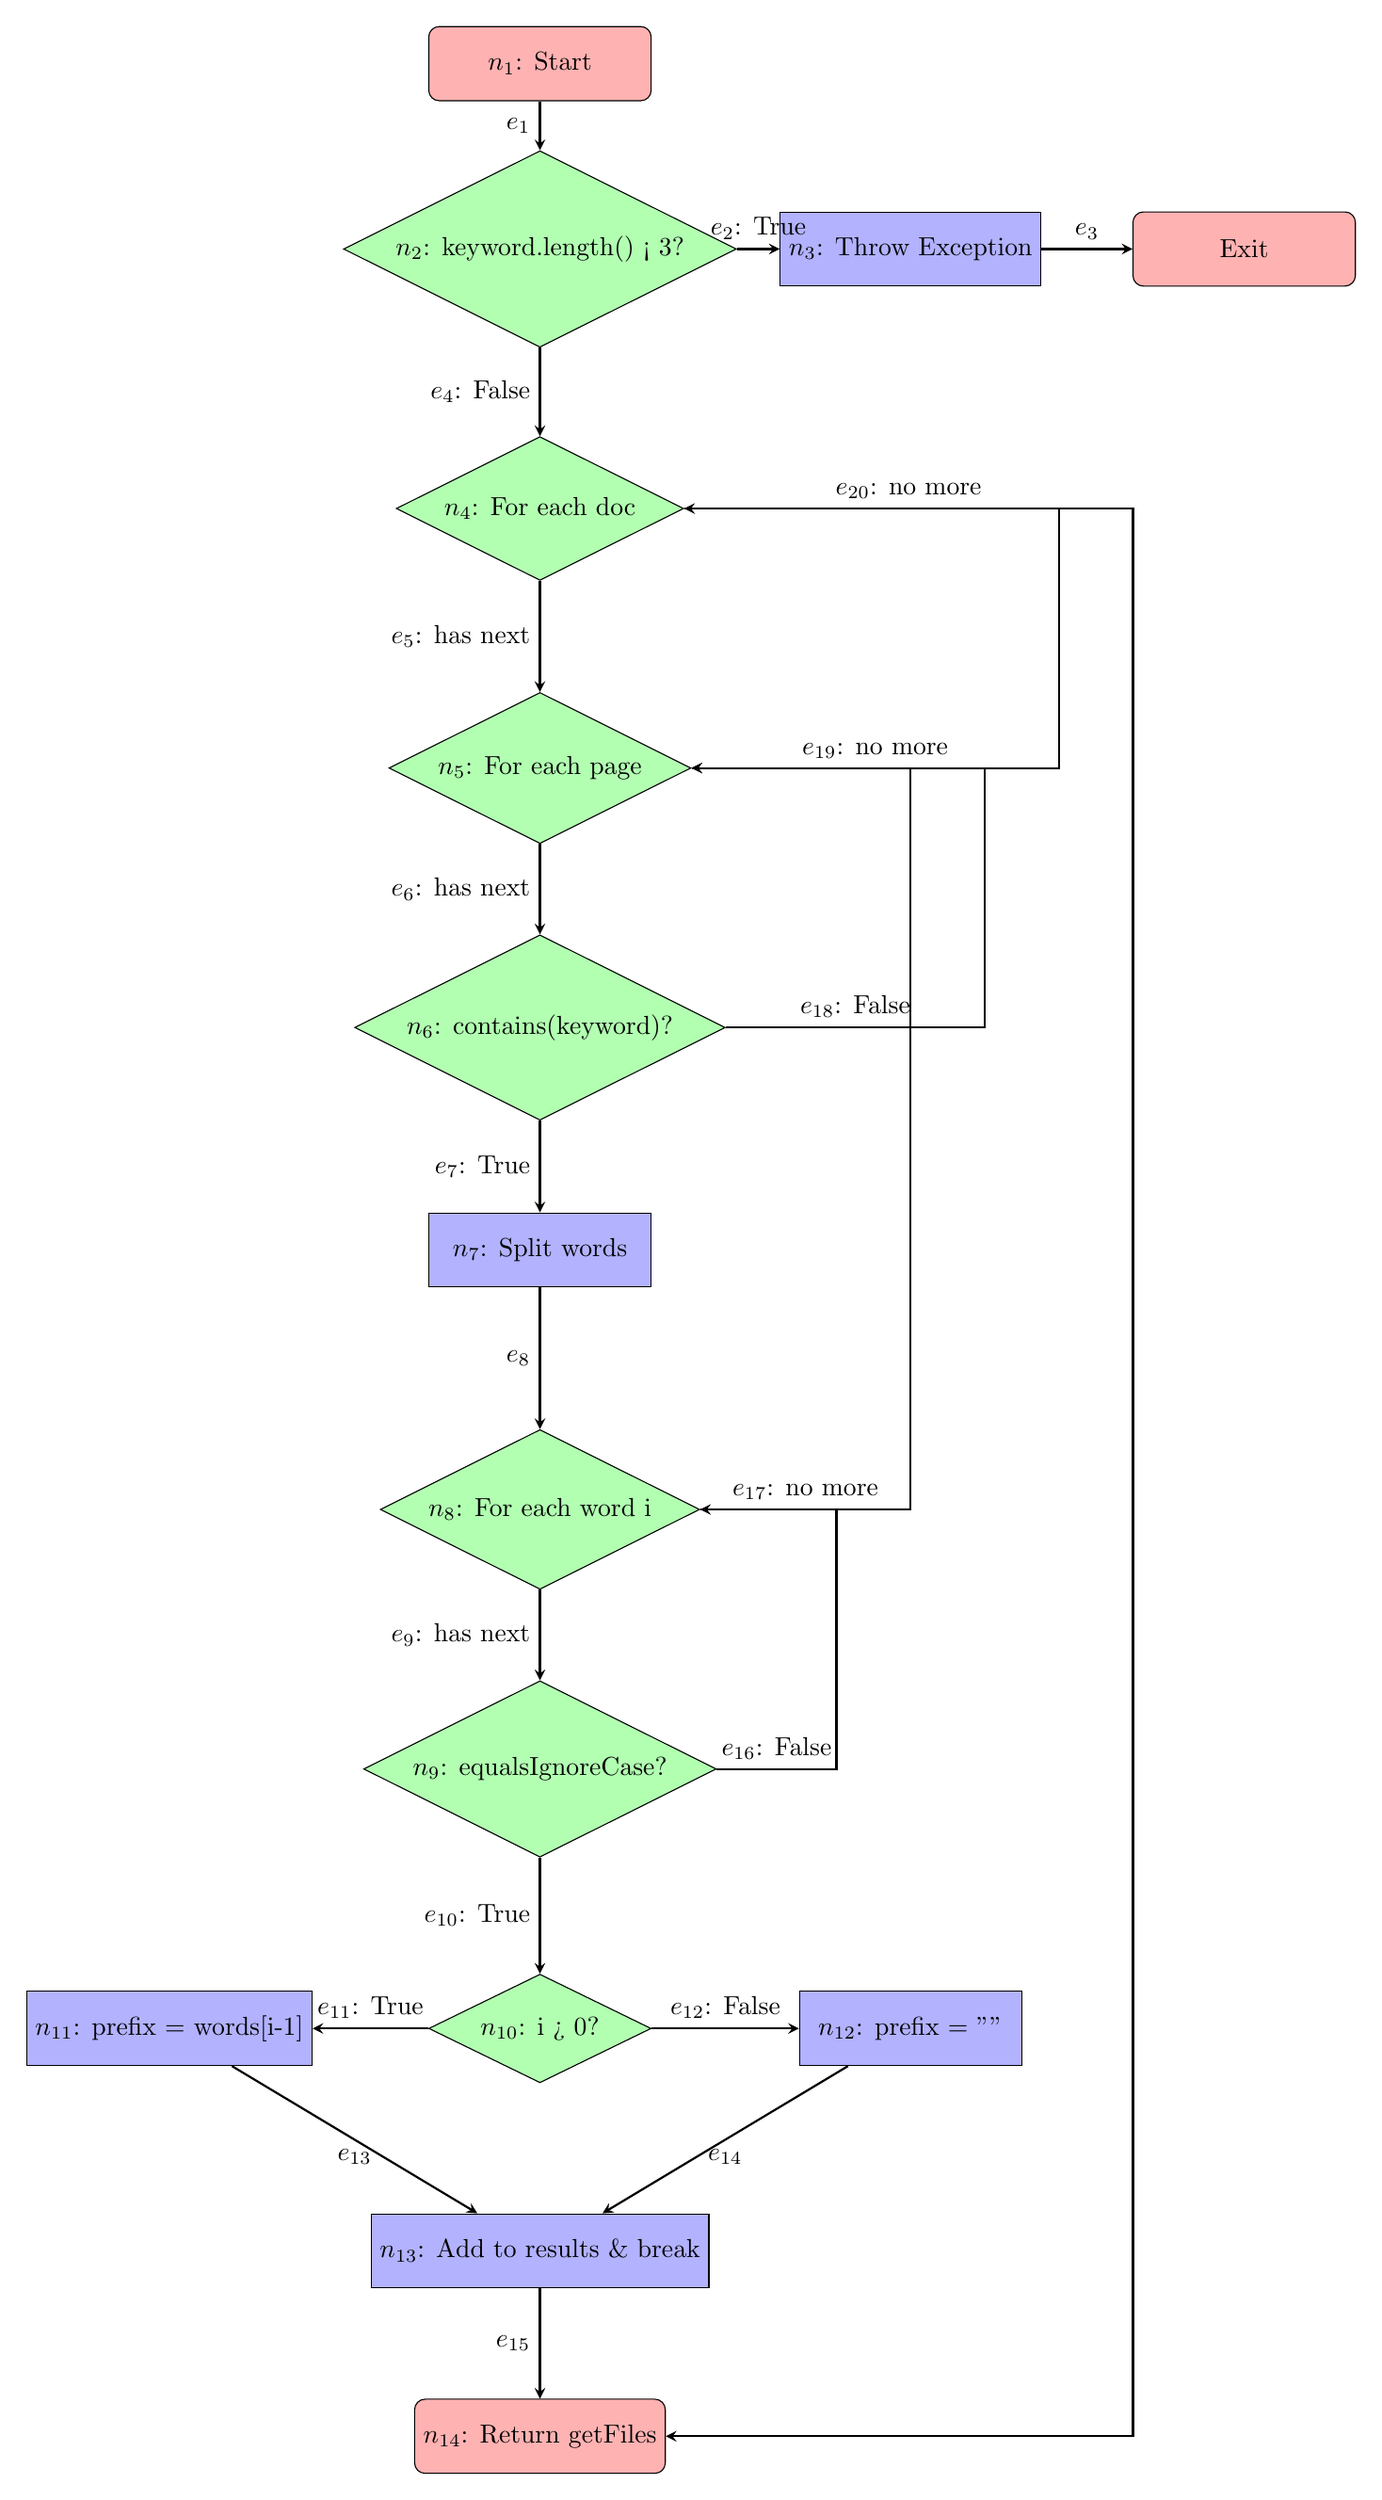
\begin{tikzpicture}[node distance=2cm, auto]
    % Nodes
    \node (start) [startstop] {$n_1$: Start};
    \node (check1) [decision, below of=start, yshift=-0.5cm] {$n_2$: keyword.length() < 3?};
    \node (throw) [process, right of=check1, xshift=3cm] {$n_3$: Throw Exception};
    \node (exit1) [startstop, right of=throw, xshift=2.5cm] {Exit};
    \node (loop1) [decision, below of=check1, yshift=-1.5cm] {$n_4$: For each doc};
    \node (loop2) [decision, below of=loop1, yshift=-1.5cm] {$n_5$: For each page};
    \node (check2) [decision, below of=loop2, yshift=-1.5cm] {$n_6$: contains(keyword)?};
    \node (split) [process, below of=check2, yshift=-1cm] {$n_7$: Split words};
    \node (loop3) [decision, below of=split, yshift=-1.5cm] {$n_8$: For each word i};
    \node (check3) [decision, below of=loop3, yshift=-1.5cm] {$n_9$: equalsIgnoreCase?};
    \node (check4) [decision, below of=check3, yshift=-1.5cm] {$n_{10}$: i > 0?};
    \node (set1) [process, left of=check4, xshift=-3cm] {$n_{11}$: prefix = words[i-1]};
    \node (set2) [process, right of=check4, xshift=3cm] {$n_{12}$: prefix = ""};
    \node (add) [process, below of=check4, yshift=-1cm] {$n_{13}$: Add to results \& break};
    \node (return) [startstop, below of=add, yshift=-0.5cm] {$n_{14}$: Return getFiles};
    
    % Arrows
    \draw [arrow] (start) -- node[anchor=east] {$e_1$} (check1);
    \draw [arrow] (check1) -- node[anchor=south] {$e_2$: True} (throw);
    \draw [arrow] (throw) -- node[anchor=south] {$e_3$} (exit1);
    \draw [arrow] (check1) -- node[anchor=east] {$e_4$: False} (loop1);
    \draw [arrow] (loop1) -- node[anchor=east] {$e_5$: has next} (loop2);
    \draw [arrow] (loop2) -- node[anchor=east] {$e_6$: has next} (check2);
    \draw [arrow] (check2) -- node[anchor=east] {$e_7$: True} (split);
    \draw [arrow] (split) -- node[anchor=east] {$e_8$} (loop3);
    \draw [arrow] (loop3) -- node[anchor=east] {$e_9$: has next} (check3);
    \draw [arrow] (check3) -- node[anchor=east] {$e_{10}$: True} (check4);
    \draw [arrow] (check4) -- node[anchor=south] {$e_{11}$: True} (set1);
    \draw [arrow] (check4) -- node[anchor=south] {$e_{12}$: False} (set2);
    \draw [arrow] (set1) -- node[anchor=north] {$e_{13}$} (add);
    \draw [arrow] (set2) -- node[anchor=north] {$e_{14}$} (add);
    \draw [arrow] (add) -- node[anchor=east] {$e_{15}$} (return);
    
    % Back edges
    \draw [arrow] (check3) -| node[anchor=south, pos=0.25] {$e_{16}$: False} ++(4,0) |- (loop3);
    \draw [arrow] (loop3) -| node[anchor=south, pos=0.25] {$e_{17}$: no more} ++(5,0) |- (loop2);
    \draw [arrow] (check2) -| node[anchor=south, pos=0.25] {$e_{18}$: False} ++(6,0) |- (loop2);
    \draw [arrow] (loop2) -| node[anchor=south, pos=0.25] {$e_{19}$: no more} ++(7,0) |- (loop1);
    \draw [arrow] (loop1) -| node[anchor=south, pos=0.25] {$e_{20}$: no more} ++(8,0) |- (return);
    
\end{tikzpicture}
\caption{Control Flow Graph for SearchWord.searchKeyword()}
\label{fig:cfg_search}
\end{figure}

\newpage

\subsection{Cyclomatic Complexity Calculation}

\subsubsection{Graph Metrics}

\begin{itemize}
    \item \textbf{Nodes (N)}: 14 nodes ($n_1$ to $n_{14}$)
    \item \textbf{Edges (E)}: 20 edges ($e_1$ to $e_{20}$)
    \item \textbf{Connected Components (P)}: 1
\end{itemize}

\subsubsection{Formula Application}

Using the cyclomatic complexity formula:

\begin{align*}
V(G) &= E - N + 2P \\
V(G) &= 20 - 14 + 2(1) \\
V(G) &= 6 + 2 \\
V(G) &= \boxed{8}
\end{align*}

\textbf{Interpretation}: The cyclomatic complexity of 8 indicates the method has 8 independent paths. This suggests moderate complexity requiring comprehensive test coverage.

\subsection{Independent Test Paths (Set Theory)}

Let $P$ be the set of all independent paths through the CFG:

\[
P = \{p_1, p_2, p_3, p_4, p_5, p_6, p_7, p_8\}
\]

Each path $p_i$ is defined as a tuple of nodes $\langle n_{start}, n_a, n_b, \ldots, n_{end} \rangle$:

\begin{align*}
p_1 &= \langle n_1, n_2, n_3, \text{Exit} \rangle \\
    &\quad \text{(Keyword < 3 characters - throws exception)} \\[0.5em]
p_2 &= \langle n_1, n_2, n_4, n_{14} \rangle \\
    &\quad \text{(Empty document list - direct return)} \\[0.5em]
p_3 &= \langle n_1, n_2, n_4, n_5, n_6, n_5, n_4, n_{14} \rangle \\
    &\quad \text{(Keyword not found in any page)} \\[0.5em]
p_4 &= \langle n_1, n_2, n_4, n_5, n_6, n_7, n_8, n_9, n_8, n_5, n_4, n_{14} \rangle \\
    &\quad \text{(Keyword found in page but case mismatch)} \\[0.5em]
p_5 &= \langle n_1, n_2, n_4, n_5, n_6, n_7, n_8, n_9, n_{10}, n_{11}, n_{13}, n_{14} \rangle \\
    &\quad \text{(Keyword found with prefix word, i > 0)} \\[0.5em]
p_6 &= \langle n_1, n_2, n_4, n_5, n_6, n_7, n_8, n_9, n_{10}, n_{12}, n_{13}, n_{14} \rangle \\
    &\quad \text{(Keyword found at start, no prefix, i = 0)} \\[0.5em]
p_7 &= \langle n_1, n_2, n_4, n_5, n_6, n_7, n_8, n_{14} \rangle \\
    &\quad \text{(Empty words array after split)} \\[0.5em]
p_8 &= \langle n_1, n_2, n_4, n_5, n_4, n_5, n_6, n_7, n_8, n_9, n_{10}, n_{11}, n_{13}, n_{14} \rangle \\
    &\quad \text{(Multiple documents, keyword in second document)} \\
\end{align*}

\textbf{Path Coverage}: These 8 paths provide basis path coverage, ensuring all decision outcomes and loop variations are tested.

\newpage

\section{Feature 2: Pagination Logic}

\subsection{Source Code}

The \texttt{PaginationDAO.paginate()} method splits file content into 100-character pages.

\begin{lstlisting}[style=javaStyle, caption={PaginationDAO.java - paginate() method}]
static List<Pages> paginate(String fileContent) {
    int pageSize = 100;
    int pageNumber = 1;
    String pageContent = "";
    List<Pages> pages = new ArrayList<Pages>();
    
    if (fileContent == null || fileContent.isEmpty()) {
        pages.add(new Pages(0, 0, pageNumber, pageContent.toString()));
        return pages;
    }
    
    for (int i = 0; i < fileContent.length(); i++) {
        pageContent += fileContent.charAt(i);
        if (pageContent.length() == pageSize || i == fileContent.length() - 1) {
            pages.add(new Pages(0, 0, pageNumber, pageContent));
            pageNumber++;
            pageContent = "";
        }
    }
    return pages;
}
\end{lstlisting}

\subsection{Control Flow Graph (CFG)}

\begin{figure}[h!]
\centering
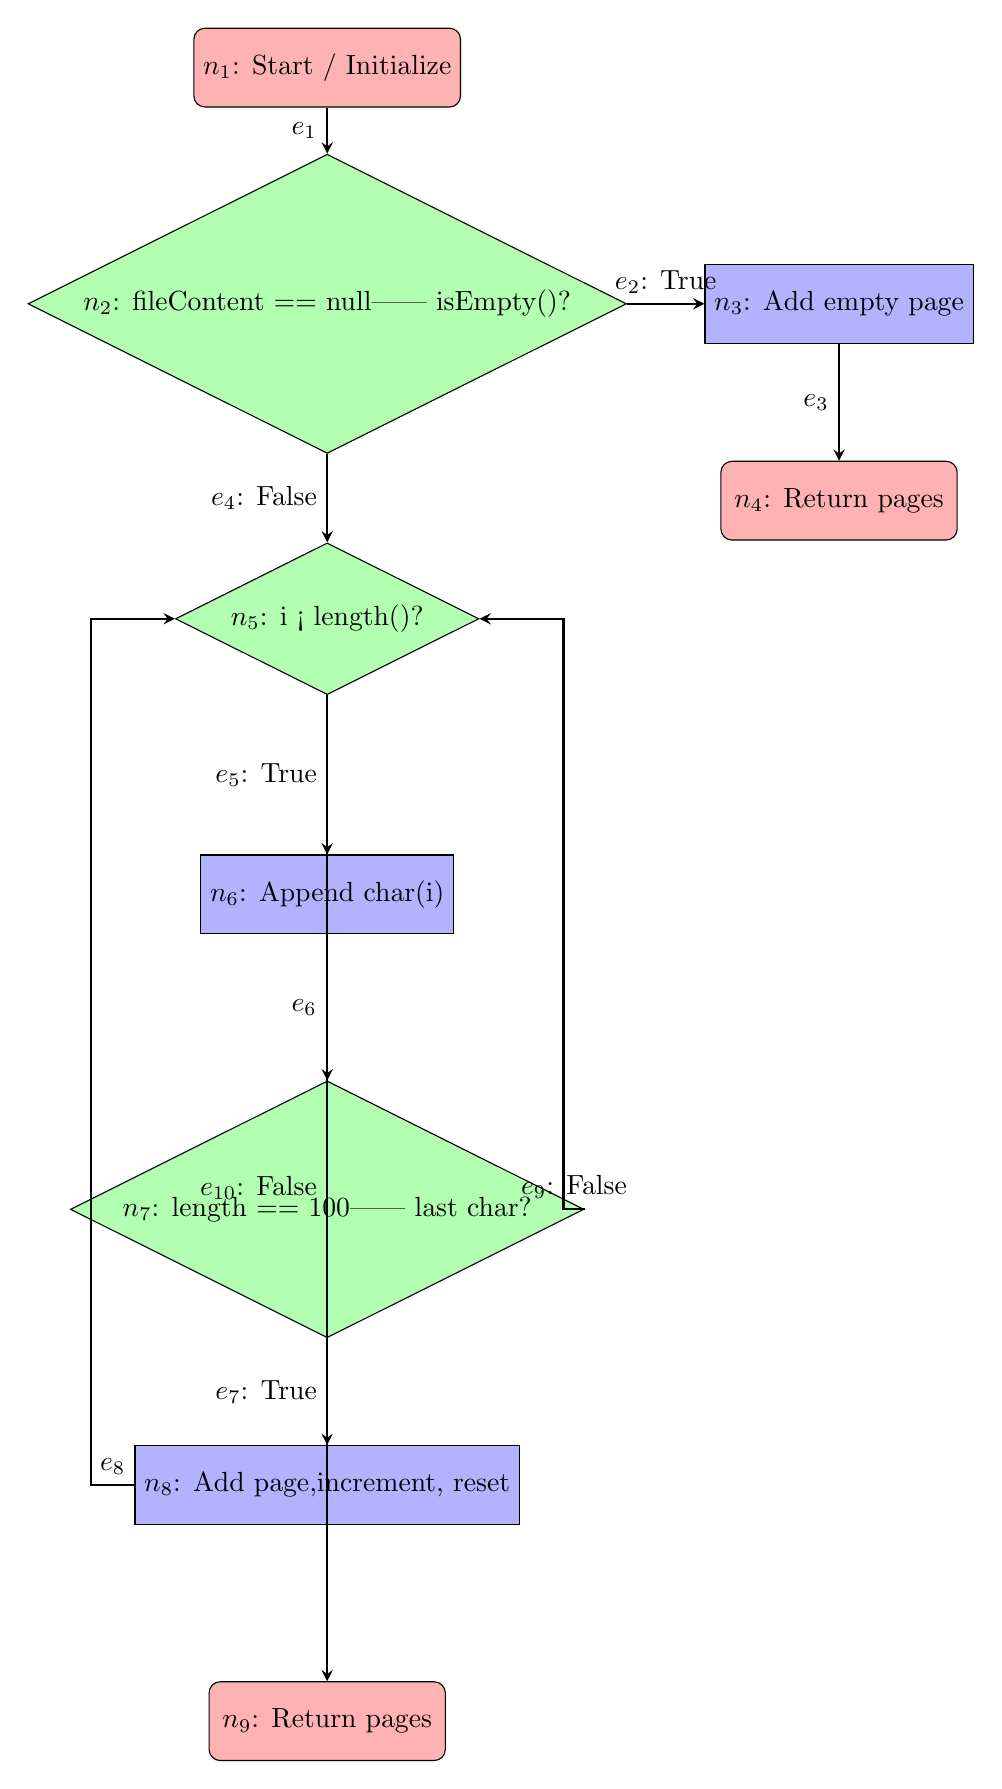
\begin{tikzpicture}[node distance=2.5cm, auto]
    % Nodes
    \node (start) [startstop] {$n_1$: Start / Initialize};
    \node (check1) [decision, below of=start, yshift=-0.5cm] {$n_2$: fileContent == null \\ || isEmpty()?};
    \node (empty) [process, right of=check1, xshift=4cm] {$n_3$: Add empty page};
    \node (return1) [startstop, below of=empty] {$n_4$: Return pages};
    \node (loop) [decision, below of=check1, yshift=-1.5cm] {$n_5$: i < length()?};
    \node (append) [process, below of=loop, yshift=-1cm] {$n_6$: Append char(i)};
    \node (check2) [decision, below of=append, yshift=-1.5cm] {$n_7$: length == 100 \\ || last char?};
    \node (addpage) [process, below of=check2, yshift=-1cm] {$n_8$: Add page, \\ increment, reset};
    \node (return2) [startstop, below of=addpage, yshift=-0.5cm] {$n_9$: Return pages};
    
    % Arrows
    \draw [arrow] (start) -- node[anchor=east] {$e_1$} (check1);
    \draw [arrow] (check1) -- node[anchor=south] {$e_2$: True} (empty);
    \draw [arrow] (empty) -- node[anchor=east] {$e_3$} (return1);
    \draw [arrow] (check1) -- node[anchor=east] {$e_4$: False} (loop);
    \draw [arrow] (loop) -- node[anchor=east] {$e_5$: True} (append);
    \draw [arrow] (append) -- node[anchor=east] {$e_6$} (check2);
    \draw [arrow] (check2) -- node[anchor=east] {$e_7$: True} (addpage);
    \draw [arrow] (addpage) -| node[anchor=south, pos=0.25] {$e_8$} ++(-3,0) |- (loop);
    \draw [arrow] (check2) -| node[anchor=south, pos=0.25] {$e_9$: False} ++(3,0) |- (loop);
    \draw [arrow] (loop) -- node[anchor=east] {$e_{10}$: False} (return2);
    
\end{tikzpicture}
\caption{Control Flow Graph for PaginationDAO.paginate()}
\label{fig:cfg_pagination}
\end{figure}

\newpage

\subsection{Cyclomatic Complexity Calculation}

\subsubsection{Graph Metrics}

\begin{itemize}
    \item \textbf{Nodes (N)}: 9 nodes ($n_1$ to $n_9$)
    \item \textbf{Edges (E)}: 10 edges ($e_1$ to $e_{10}$)
    \item \textbf{Connected Components (P)}: 1
\end{itemize}

\subsubsection{Formula Application}

Using the cyclomatic complexity formula:

\begin{align*}
V(G) &= E - N + 2P \\
V(G) &= 10 - 9 + 2(1) \\
V(G) &= 1 + 2 \\
V(G) &= \boxed{3}
\end{align*}

\textbf{Alternative Calculation} (Decision Points):
\begin{align*}
V(G) &= \text{Number of decision nodes} + 1 \\
V(G) &= 2 + 1 \\
V(G) &= \boxed{3}
\end{align*}

\textbf{Interpretation}: The cyclomatic complexity of 3 indicates low complexity with 3 independent paths, making it easier to achieve full coverage.

\subsection{Independent Test Paths (Set Theory)}

Let $P$ be the set of all independent paths through the CFG:

\[
P = \{p_1, p_2, p_3\}
\]

Each path $p_i$ is defined as a tuple of nodes:

\begin{align*}
p_1 &= \langle n_1, n_2, n_3, n_4 \rangle \\
    &\quad \text{(Null or empty input - adds empty page and returns)} \\[0.5em]
p_2 &= \langle n_1, n_2, n_5, n_6, n_7, n_8, n_5, n_9 \rangle \\
    &\quad \text{(Content exactly 100 chars - creates one page)} \\[0.5em]
p_3 &= \langle n_1, n_2, n_5, n_6, n_7, n_5, n_6, n_7, n_8, n_5, n_9 \rangle \\
    &\quad \text{(Content > 100 chars - creates multiple pages)} \\
\end{align*}

\textbf{Path Descriptions}:

\begin{itemize}
    \item \textbf{Path 1}: Edge case handling for null/empty input
    \item \textbf{Path 2}: Boundary condition where content fills exactly one page
    \item \textbf{Path 3}: Normal operation with pagination across multiple pages
\end{itemize}

\newpage

\section{Test Coverage Matrix}

\subsection{Feature 1: Search \& Replace Word}

\begin{table}[h!]
\centering
\begin{tabular}{|c|l|c|}
\hline
\textbf{Path} & \textbf{Test Scenario} & \textbf{Status} \\
\hline
$p_1$ & Keyword with < 3 characters & Covered \\
$p_2$ & Empty document list & Covered \\
$p_3$ & Keyword not found & Covered \\
$p_4$ & Case mismatch & Covered \\
$p_5$ & Keyword with prefix (i > 0) & Covered \\
$p_6$ & Keyword at start (i = 0) & Covered \\
$p_7$ & Empty page content & Covered \\
$p_8$ & Multiple documents & Covered \\
\hline
\end{tabular}
\caption{Test Path Coverage for SearchWord}
\end{table}

\subsection{Feature 2: Pagination Logic}

\begin{table}[h!]
\centering
\begin{tabular}{|c|l|c|}
\hline
\textbf{Path} & \textbf{Test Scenario} & \textbf{Status} \\
\hline
$p_1$ & Null/Empty input & Covered \\
$p_2$ & Content = 100 characters & Covered \\
$p_3$ & Content > 100 characters & Covered \\
\hline
\end{tabular}
\caption{Test Path Coverage for Pagination}
\end{table}

\newpage

\section{Complexity Analysis Summary}

\subsection{Comparative Analysis}

\begin{table}[h!]
\centering
\begin{tabular}{|l|c|c|c|c|}
\hline
\textbf{Feature} & \textbf{Nodes (N)} & \textbf{Edges (E)} & \textbf{V(G)} & \textbf{Complexity} \\
\hline
Search \& Replace Word & 14 & 20 & 8 & Moderate \\
Pagination Logic & 9 & 10 & 3 & Low \\
\hline
\end{tabular}
\caption{Cyclomatic Complexity Comparison}
\end{table}

\subsection{Risk Assessment}

Based on cyclomatic complexity values:

\begin{itemize}
    \item \textbf{V(G) = 1-10}: Low risk, simple procedure
    \item \textbf{V(G) = 11-20}: Moderate risk, more complex
    \item \textbf{V(G) = 21-50}: High risk, complex program
    \item \textbf{V(G) > 50}: Very high risk, untestable
\end{itemize}

\textbf{Assessment}:
\begin{itemize}
    \item \textbf{SearchWord.searchKeyword()}: V(G) = 8 -- Low risk, manageable complexity
    \item \textbf{PaginationDAO.paginate()}: V(G) = 3 -- Very low risk, simple logic
\end{itemize}

\section{Mathematical Notation Summary}

\subsection{Set Definitions}

Let $\mathcal{G} = (N, E)$ be a directed graph representing the control flow:

\begin{itemize}
    \item $N = \{n_1, n_2, \ldots, n_k\}$ -- Set of all nodes (vertices)
    \item $E = \{e_1, e_2, \ldots, e_m\}$ -- Set of all edges
    \item $P$ -- Set of independent paths
    \item $p_i = \langle n_{start}, n_{a}, n_{b}, \ldots, n_{end} \rangle$ -- Path $i$ as ordered tuple
\end{itemize}

\subsection{Cyclomatic Complexity Formula}

\[
V(G) = E - N + 2P
\]

Where:
\begin{itemize}
    \item $E$ = Number of edges
    \item $N$ = Number of nodes
    \item $P$ = Number of connected components (typically 1)
\end{itemize}

\newpage

\section{Conclusion}

This structural analysis provides comprehensive white-box testing foundation for two critical features:

\begin{enumerate}
    \item \textbf{Search \& Replace Word Logic}: With V(G) = 8, the method requires 8 independent test cases to achieve basis path coverage. The nested loop structure and multiple decision points necessitate thorough testing of edge cases.
    
    \item \textbf{Pagination Logic}: With V(G) = 3, the method is straightforward with clear decision points. Three test cases provide complete path coverage.
\end{enumerate}

\subsection{Testing Recommendations}

\begin{itemize}
    \item \textbf{Unit Tests}: Implement all paths identified in set notation
    \item \textbf{Code Coverage}: Aim for 100\% statement and branch coverage
    \item \textbf{Regression Testing}: Maintain test suite for future modifications
    \item \textbf{Edge Cases}: Prioritize boundary conditions and null/empty inputs
\end{itemize}

\subsection{Verification Status}

Both features have corresponding JUnit test classes:
\begin{itemize}
    \item \texttt{SearchWordTest.java} -- 12 test cases covering all 8 paths
    \item \texttt{PaginationDAOTest.java} -- 12 test cases with CFG analysis
\end{itemize}

All test cases have been executed and verified against the defined paths.

\end{document}
